\section{Summary}

\begin{wideslide}[toc=Neutrino interactions]{Neutrino-nucleus interactions}
\null\vfill

  \sep

  For all channels (but coherent) neutrino interactions are factorized in the following way
  
  \sep\sep\sep
  
  \centering\begin{tikzpicture}
 
  \draw [rounded corners] (0,0) -- (2,0) -- (2,2) -- (0,2) -- cycle;
  \draw [rounded corners] (2.5,0) -- (4.5,0) -- (4.5,2) -- (2.5,2) -- cycle;
  \draw [rounded corners] (5,0) -- (7,0) -- (7,2) -- (5,2) -- cycle;
  \draw [rounded corners] (7.5,0) -- (9.5,0) -- (9.5,2) -- (7.5,2) -- cycle;
  \draw [rounded corners] (10,0) -- (12,0) -- (12,2) -- (10,2) -- cycle;
  
  \draw (1,1) circle (0.75cm);
  
  \draw [filled=pdcolor4, draw=none] (1.1, 1.2) circle (0.1cm);    
  \draw [filled=pdcolor5, draw=none] (1.4, 1.3) circle (0.1cm);    
  \draw [filled=pdcolor4, draw=none] (1.5, 0.9) circle (0.1cm);    
  \draw [filled=pdcolor5, draw=none] (1.3, 0.6) circle (0.1cm);    
  \draw [filled=pdcolor4, draw=none] (0.8, 1.4) circle (0.1cm);    
  \draw [filled=pdcolor5, draw=none] (0.5, 1.0) circle (0.1cm);    
  \draw [filled=pdcolor4, draw=none] (0.8, 0.7) circle (0.1cm);
  
  \draw (3,0.5) -- (3.5,1) -- (3,1.5);
  \draw [curl] (3.5,1) -- (4.1,1);
  \draw [filled=pdcolor1, draw=none] (3,0.5) circle (0.1cm);
  \draw [filled=pdcolor1, draw=none] (3,1.5) circle (0.1cm);
  \draw [filled=pdcolor4, draw=none] (4.1,1) circle (0.1cm);
  
  \node at (6,1) {\scalebox{0.2}{\begin{tikzpicture}
  
  \node (center) {};
  
  \node [circle, filled={pdcolor4}, minimum width = 1cm, below=of center, xshift = 3cm, yshift = 0cm] {}; 
  \node [circle, filled={pdcolor5}, minimum width = 1cm, below=of center, xshift = 6cm, yshift = 1cm] {}; 
  \node [circle, filled={pdcolor6}, minimum width = 1cm, below=of center, xshift = 2cm, yshift = 2cm] {}; 
  \node [circle, filled={pdcolor7}, minimum width = 1cm, below=of center, xshift = 0cm, yshift = 3cm] {}; 
  \node [circle, filled={pdcolor4}, minimum width = 1cm, below=of center, xshift = 1cm, yshift = 4cm] {}; 
  \node [circle, filled={pdcolor5}, minimum width = 1cm, below=of center, xshift = 4cm, yshift = 3.5cm] {}; 
  \node [circle, filled={pdcolor6}, minimum width = 1cm, below=of center, xshift = 2.5cm, yshift = 3.5cm] {}; 
  \node [circle, filled={pdcolor7}, minimum width = 1cm, below=of center, xshift = 4.25cm, yshift = 1.5cm] {}; 
 
\end{tikzpicture}
}};
 
  \foreach \x in {1,...,10}
  {
    \pgfmathsetmacro{\r}{\x / 100}
    \pgfmathsetmacro{\o}{\x / 10}
    \draw [filled=pdcolor1, draw=none, fill opacity = \o] (8 + \o, 1) circle (\r cm);  
    \draw [filled=pdcolor4, draw=none, fill opacity = \o] (8 + \o, 1 + \o / 2) circle (\r cm);  
    \draw [filled=pdcolor6, draw=none, fill opacity = \o] (8 + \o, 1 - \o / 2) circle (\r cm);  
  }
  
  \node [below] at (1.0, 0) {IA};
  \node [below] at (3.5, 0) {$\nu N$};
  \node [below] at (6.0, 0) {hadronization};
  \node [below] at (8.5, 0) {formation time};
  \node [below] at (11., 0) {FSI};
  
  \node at (11,1) {\scalebox{0.2}{\tikzset{
p/.style = {ultra thick, color = pdcolor1, >=latex, ->},
n/.style = {ultra thick, color = pdcolor4, >=latex, ->},
pi/.style = {ultra thick, color = pdcolor5, >=latex, ->},
pip/.style = {ultra thick, color = pdcolor6, >=latex, ->},
pim/.style = {ultra thick, color = pdcolor7, >=latex, ->},
}

\begin{tikzpicture}
    
    \draw[n] (-2,0) -- node[left] {$n$} (-1,1.5);
    \draw[p] (-1,1.5) -- (-1, 3.5) node[left] {$p$};
    \draw[n] (-1,1.5) -- node[above] {$n$} (0,1.5);
    \draw[p] (0,1.5) -- (2.5,3) node[above] {$p$};
    \draw[pim] (0, 1.5) -- node[above] {$\pi^-$} (1.5, 0.5);
    \draw[pim] (1.5, 0.5) -- (3.75, 0.25) node[above] {$\pi^-$};
    \draw[n] (1.5, 0.5) -- node[right] {$n$} (1.75, -0.5);
    
    \draw[pip] (-2,0) -- node[above] {$\pi^+$} (-0.5,0);
    \draw[p] (-0.5,0) -- node[above] {$p$} (0, 0.5);
    \draw[pi] (-0.5,0) -- node[above] {$\pi^0$} (1,-1);
    \draw[n] (1,-1) -- (3.5,-1.5) node[above] {$n$};
    \draw[p] (1,-1) -- (2.75, -2.75) node [right] {$p$};
    
    \draw[pi] (-2,0) -- node[left] {$\pi^0$} (-1,-1.5);
    \draw[pim] (-1,-1.5) -- (-1.5, -3.5) node[right] {$\pi^-$};
    \draw[pip] (-1,-1.5) -- (0, -3.5) node[right] {$\pi^+$};
    \draw[n] (-1,-1.5) -- node[above] {$n$} (0, -2);
    \draw[n] (0,-2) -- node[above] {$n$} (1, -1.5);
    \draw[p] (0,-2) -- node[below] {$p$} (1, -2.5);
    
    \draw[ultra thick, color = pdcolor1] (0,0) circle (3);
    
    \draw[ultra thick, color = pdcolor1, >=latex, ->] (-4, 0) -- (-2,0);

\end{tikzpicture}
}};
 
\end{tikzpicture}

  
  \sep\sep
  
  \begin{itemize}
   \item Is the physics really factorized this way?
   \item This factorization is common for all generators
   \item However, some pieces are done in different way
  \end{itemize}
  
\vfill\null
\end{wideslide}

\begin{slide}[toc=MiniBooNE CC $\pi$]{MiniBooNE data for CC $\pi$ production}

  \rput(12, 4.25)
  {
  \begin{pspicture}
   
    \pscircle[linestyle = none, fillstyle = solid, fillcolor = pdcolor1](0,0){1}

    \pscircle[linestyle = none, fillstyle = solid, fillcolor = pdcolor4](-2.5,0){0.2}
    \psline[linewidth = 0.05, linecolor = pdcolor4]{->}(-2.1,0)(-1.2,0)
    \rput[c](-1.75,0.25){\color{pdcolor4}\small $\left<E_\nu\right>$}
    \rput[c](-1.75,-0.24){\color{pdcolor4}\small $\sim 1$~GeV}
    \psline[linewidth = 0.05, linecolor = pdcolor1]{->}(1.2,0)(1.6,0)
    
    \rput[l](2,0.75){\color{pdcolor1} 1$\mu$}
    \rput[l](2,0){\color{pdcolor1} 0$\pi^\pm$ (0$\pi^{\overset{0}{-}}$)}
    \rput[l](2,-0.75){\color{pdcolor1} 1$\pi^0$ (1$\pi^+$)}
    
  \end{pspicture}
  }

  \begin{itemize}
   
   \item The cross section \\ for $\pi^0$ ($\pi^+$) production \\ through charge current \\ measured by MiniBooNE
   
   \item The signal is defined as: charged leptons, no charged pions and one neutral pion (one positive pion and no other pions) in the final state.
   
   \item The result depends on primary vertex and FSI, as pion can be:
   
   \vspace{5pt}
   
    \begin{itemize}
    
      \item produced in primary vertex
      \item produced in FSI
      \item affected by charge exchange
      \item absorbed
    
    \end{itemize}
    
  \end{itemize}
  
\end{slide}

\begin{wideslide}[toc=]{MiniBooNE data for CC $\pi$ production}
\null\vfill

  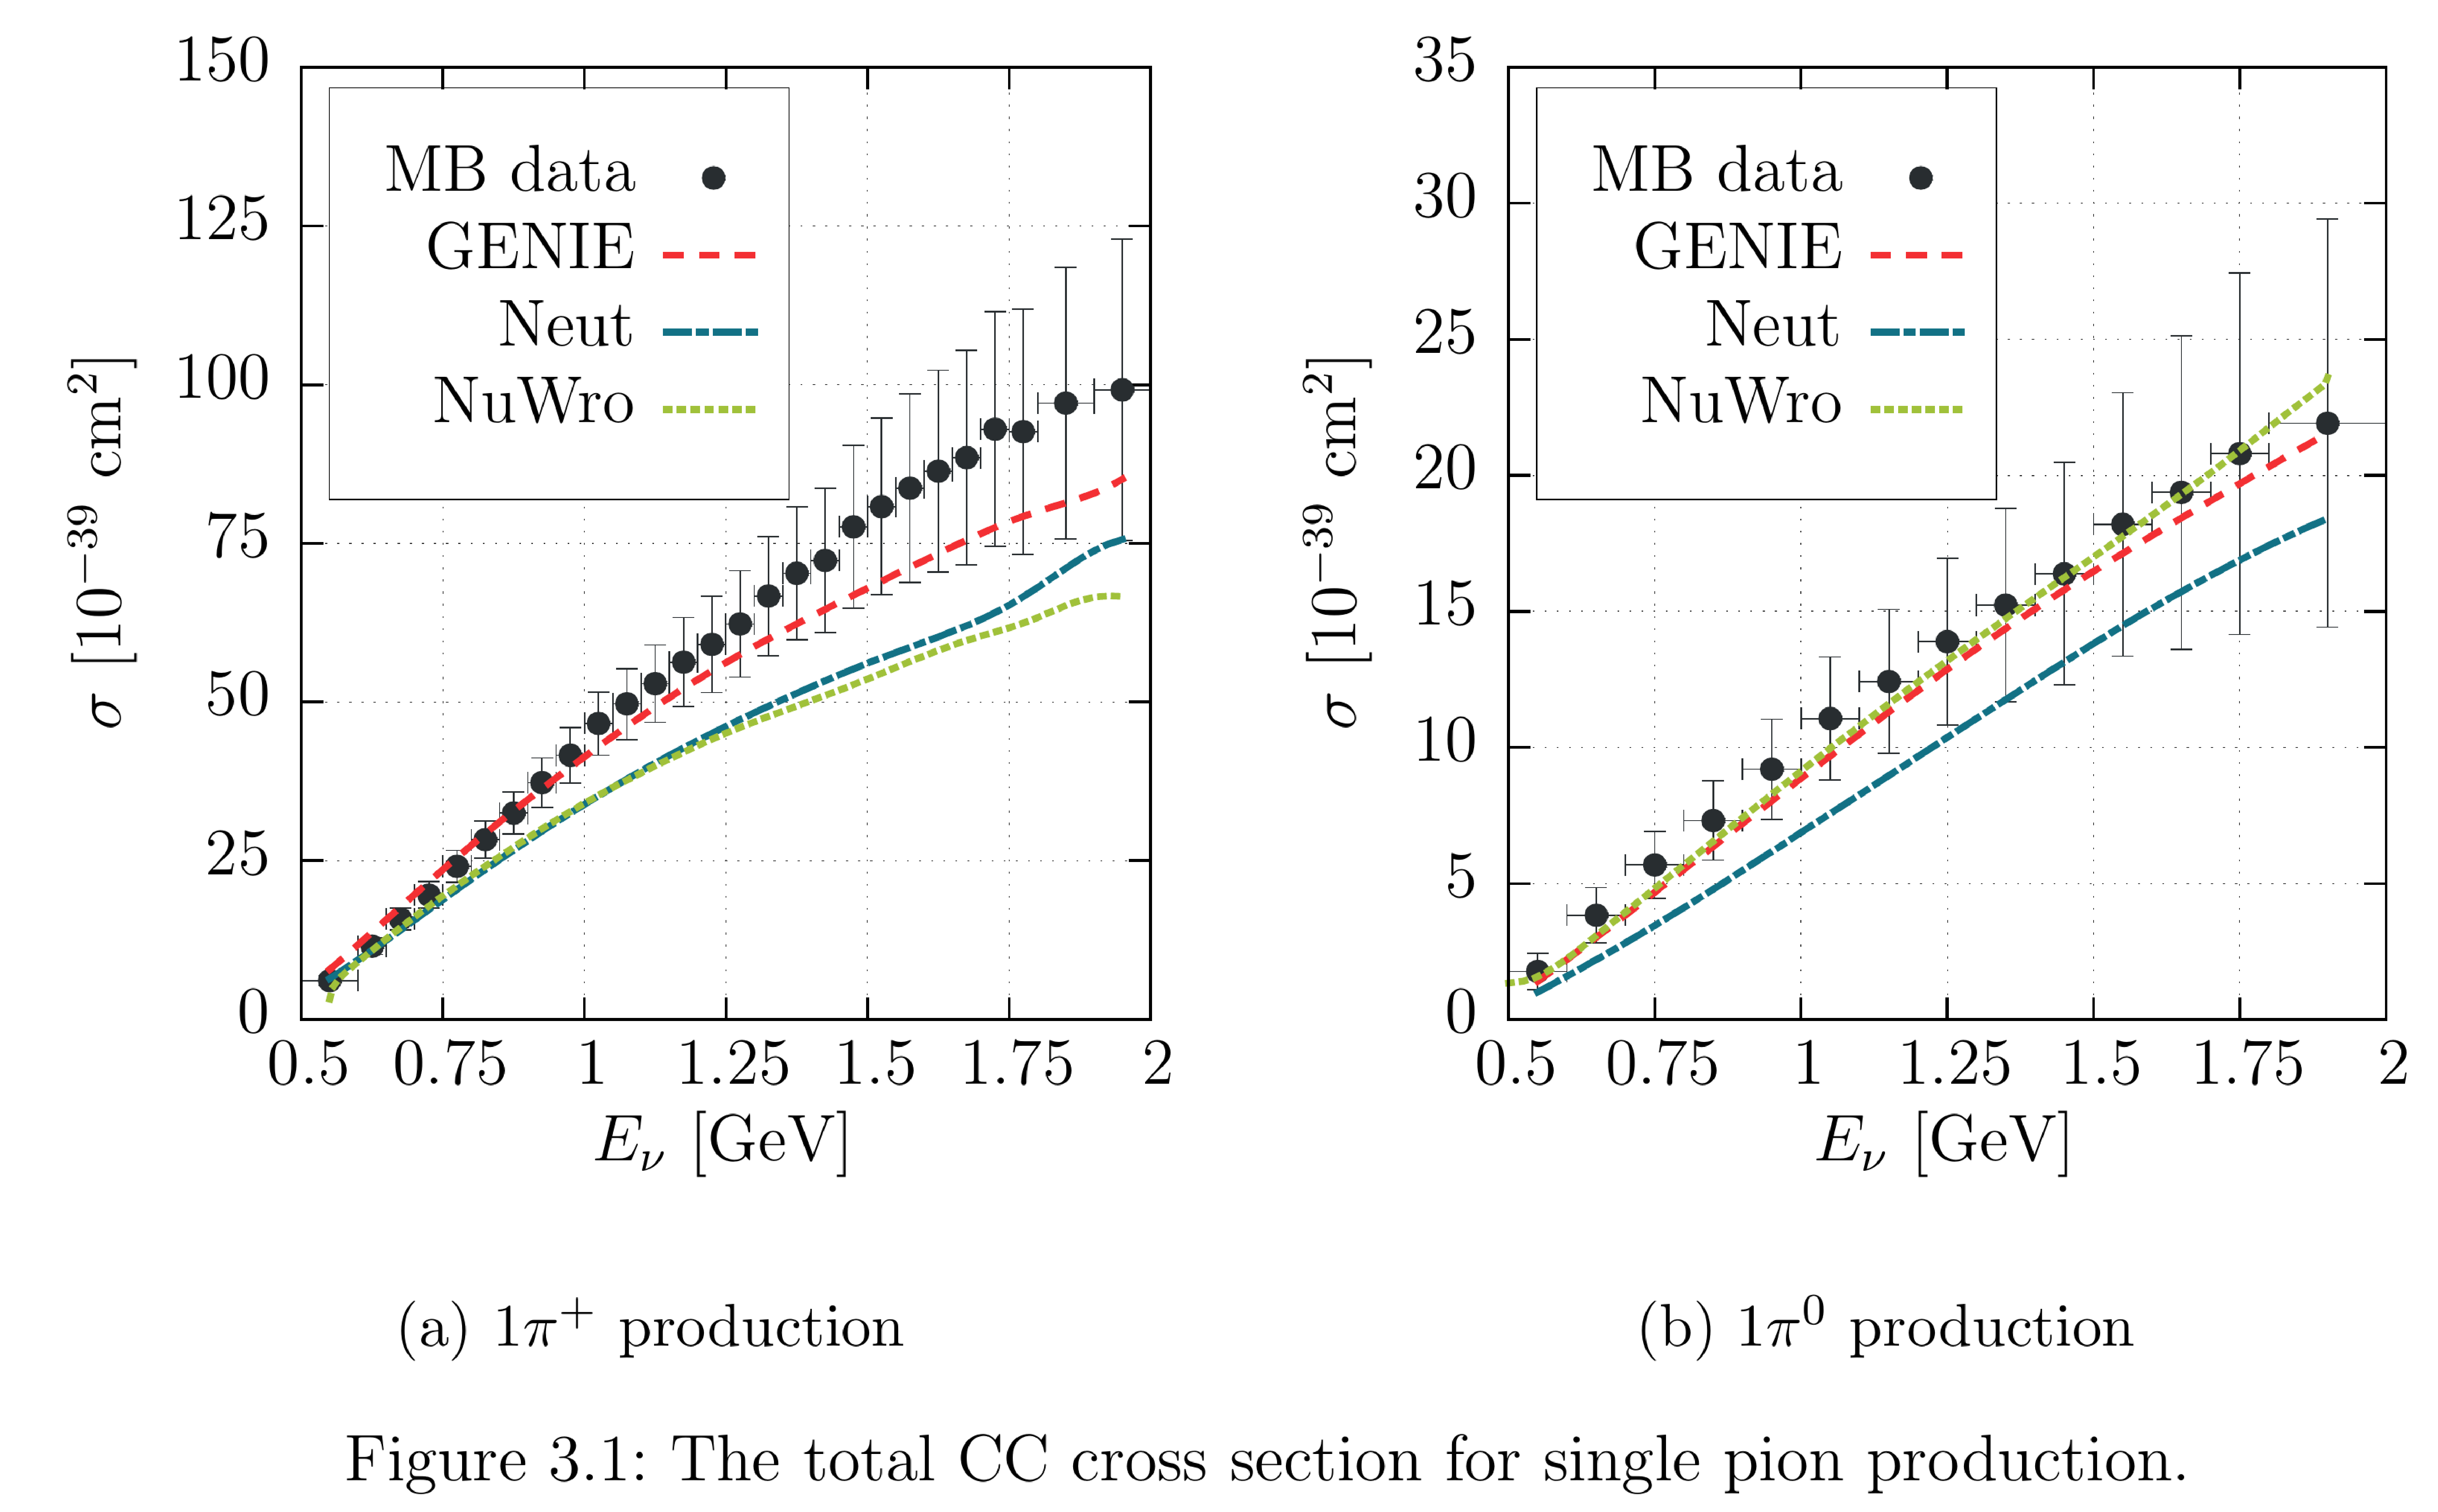
\includegraphics[width=\columnwidth]{figures/mbtot.eps}

\vfill\null
\end{wideslide}

\begin{wideslide}[toc=]{MiniBooNE data for CC $\pi$ production}
\null\vfill

  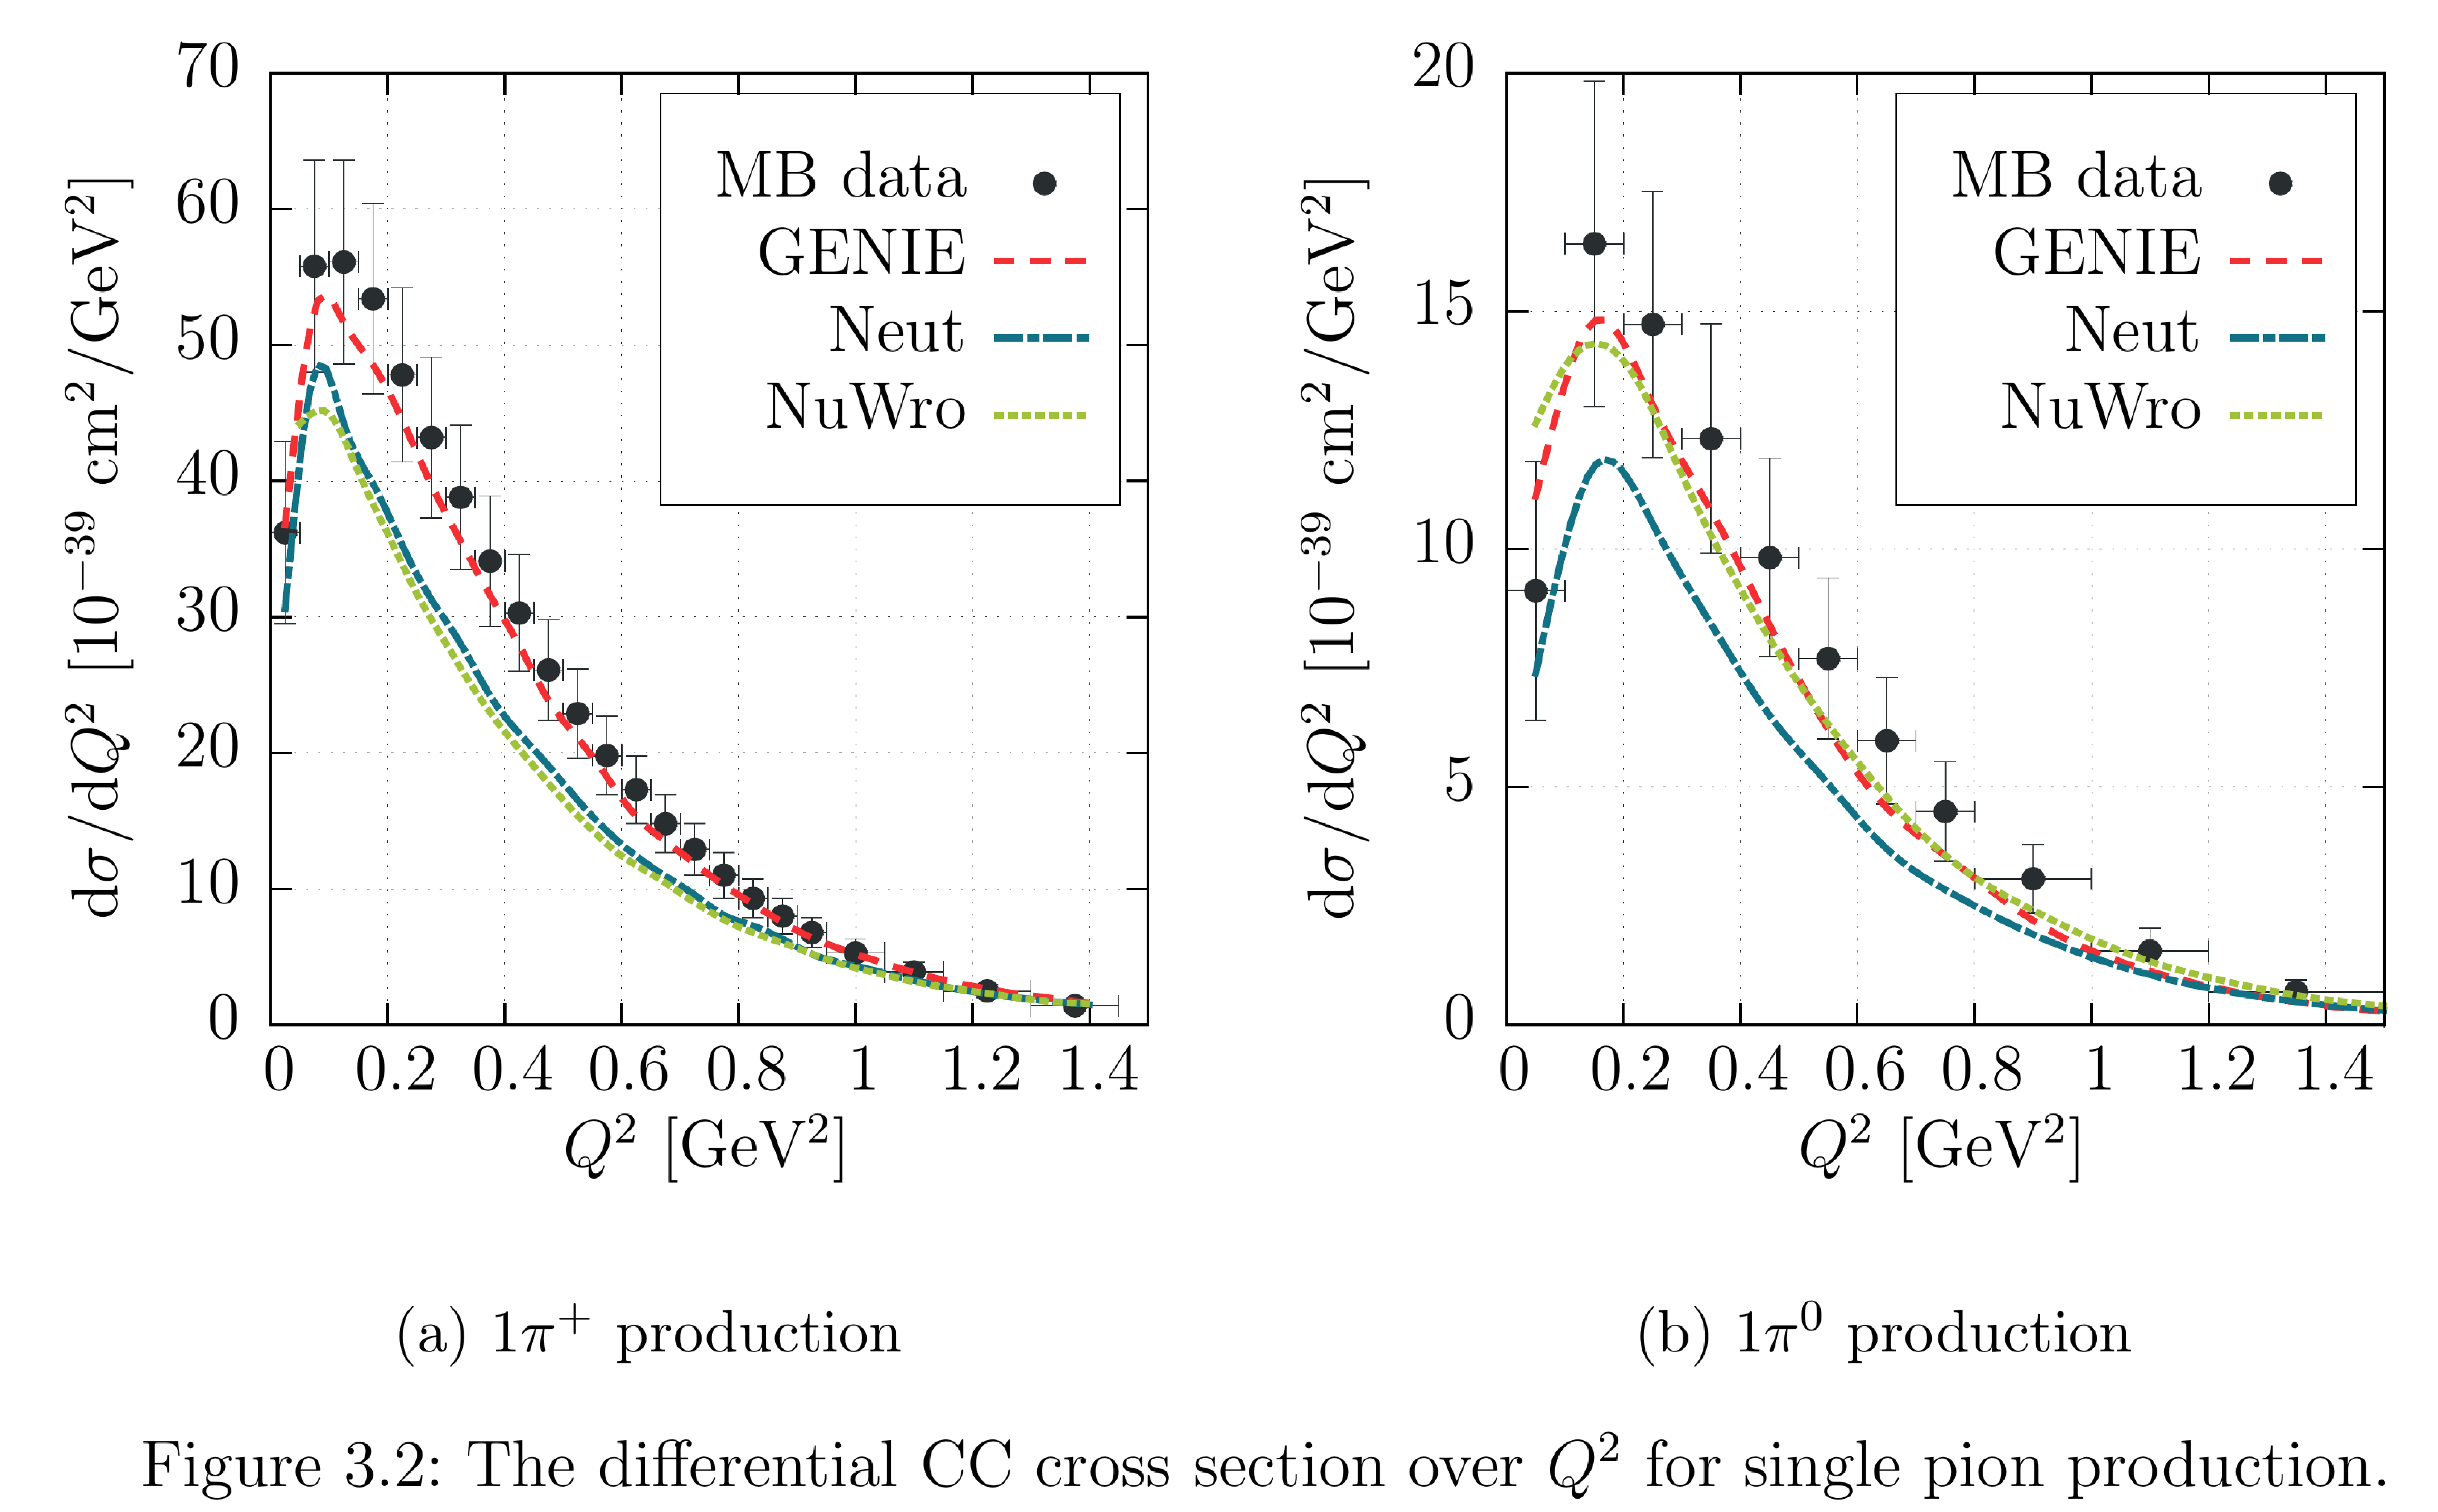
\includegraphics[width=\columnwidth]{figures/mbq2.eps}

\vfill\null
\end{wideslide}

\begin{slide}{Summary}
\null\vfill

  \rput(1.1\slidewidth, 0.55\slideheight){\scalebox{1.5}{\begin{pspicture}
  \pscircle[linewidth = 0.05, linecolor = pdcolor1](0,0){1}

  \psline[linewidth = 0.05, linecolor = pdcolor4]{->}(-1.6,0)(-1.1,0)
  \psline[linewidth = 0.05, linecolor = pdcolor5]{->}(1.1,0.5)(1.6,0.75)
  \psline[linewidth = 0.05, linecolor = pdcolor5]{->}(1.1,0)(1.6,0)
  \psline[linewidth = 0.05, linecolor = pdcolor5]{->}(1.1,-0.5)(1.6,-0.75)
  
  \rput[c](0,0){\scalebox{0.075}{%LaTeX with PSTricks extensions
%%Creator: inkscape 0.48.4
%%Please note this file requires PSTricks extensions
\psset{xunit=.5pt,yunit=.5pt,runit=.5pt}
\begin{pspicture}(1024,1024)
{
\newrgbcolor{curcolor}{0.12941177 0.14509805 0.19607843}
\pscustom[linestyle=none,fillstyle=solid,fillcolor=curcolor]
{
\newpath
\moveto(476.52942,979.76519)
\curveto(487.77942,998.51519)(514.02942,1021.01519)(532.77942,1021.01519)
\lineto(945.27942,788.51519)
\curveto(952.77942,781.01519)(971.52942,732.26519)(956.52942,713.51519)
\lineto(547.77942,473.51519)
\curveto(536.52942,469.76519)(487.77942,473.51519)(472.77942,511.01519)
\lineto(476.52942,979.76519)
\closepath
}
}
{
\newrgbcolor{curcolor}{0.12941177 0.14509805 0.19607843}
\pscustom[linewidth=3,linecolor=curcolor]
{
\newpath
\moveto(476.52942,979.76519)
\curveto(487.77942,998.51519)(514.02942,1021.01519)(532.77942,1021.01519)
\lineto(945.27942,788.51519)
\curveto(952.77942,781.01519)(971.52942,732.26519)(956.52942,713.51519)
\lineto(547.77942,473.51519)
\curveto(536.52942,469.76519)(487.77942,473.51519)(472.77942,511.01519)
\lineto(476.52942,979.76519)
\closepath
}
}
{
\newrgbcolor{curcolor}{1 1 1}
\pscustom[linestyle=none,fillstyle=solid,fillcolor=curcolor]
{
\newpath
\moveto(517.1383,502.04801)
\curveto(506.42376,483.44891)(488.892,483.44915)(478.17747,502.04825)
\lineto(359.4827,708.08751)
\curveto(348.76859,726.68588)(348.76816,757.11932)(359.4827,775.7184)
\lineto(478.17747,981.75767)
\curveto(488.89172,1000.356275)(506.42418,1000.356275)(517.1383,981.75791)
\lineto(635.83307,775.71865)
\curveto(646.54761,757.11956)(646.54732,726.68588)(635.83307,708.08728)
\lineto(517.1383,502.04801)
\closepath
}
}
{
\newrgbcolor{curcolor}{0.12941177 0.14509805 0.19607843}
\pscustom[linewidth=3.73868561,linecolor=curcolor]
{
\newpath
\moveto(517.1383,502.04801)
\curveto(506.42376,483.44891)(488.892,483.44915)(478.17747,502.04825)
\lineto(359.4827,708.08751)
\curveto(348.76859,726.68588)(348.76816,757.11932)(359.4827,775.7184)
\lineto(478.17747,981.75767)
\curveto(488.89172,1000.356275)(506.42418,1000.356275)(517.1383,981.75791)
\lineto(635.83307,775.71865)
\curveto(646.54761,757.11956)(646.54732,726.68588)(635.83307,708.08728)
\lineto(517.1383,502.04801)
\closepath
}
}
{
\newrgbcolor{curcolor}{0.12941177 0.14509805 0.19607843}
\pscustom[linestyle=none,fillstyle=solid,fillcolor=curcolor]
{
\newpath
\moveto(514.02984324,770.32250396)
\curveto(523.07178558,754.62682324)(523.07178558,729.17909676)(514.02984324,713.48341604)
\curveto(504.98790089,697.78773531)(490.32801581,697.78773531)(481.28607346,713.48341604)
\curveto(472.24413112,729.17909676)(472.24413112,754.62682324)(481.28607346,770.32250396)
\curveto(490.32801581,786.01818469)(504.98790089,786.01818469)(514.02984324,770.32250396)
\closepath
}
}
{
\newrgbcolor{curcolor}{0.12941177 0.14509805 0.19607843}
\pscustom[linewidth=2.67048985,linecolor=curcolor]
{
\newpath
\moveto(514.02984324,770.32250396)
\curveto(523.07178558,754.62682324)(523.07178558,729.17909676)(514.02984324,713.48341604)
\curveto(504.98790089,697.78773531)(490.32801581,697.78773531)(481.28607346,713.48341604)
\curveto(472.24413112,729.17909676)(472.24413112,754.62682324)(481.28607346,770.32250396)
\curveto(490.32801581,786.01818469)(504.98790089,786.01818469)(514.02984324,770.32250396)
\closepath
}
}
{
\newrgbcolor{curcolor}{1 1 1}
\pscustom[linestyle=none,fillstyle=solid,fillcolor=curcolor]
{
\newpath
\moveto(936.13332,746.70165)
\curveto(957.59787,746.72225)(966.36354,731.53907)(955.61352,712.96046)
\lineto(836.52566,507.14816)
\curveto(825.77606,488.57028)(799.42013,473.35319)(777.95558,473.33272)
\lineto(540.17294,473.10577)
\curveto(518.70894,473.08527)(509.9427,488.26883)(520.6923,506.8467)
\lineto(639.78018,712.65902)
\curveto(650.5302,731.23763)(676.88668,746.45421)(698.35068,746.4747)
\lineto(936.13332,746.70165)
\closepath
}
}
{
\newrgbcolor{curcolor}{0.12941177 0.14509805 0.19607843}
\pscustom[linewidth=3.73868561,linecolor=curcolor]
{
\newpath
\moveto(936.13332,746.70165)
\curveto(957.59787,746.72225)(966.36354,731.53907)(955.61352,712.96046)
\lineto(836.52566,507.14816)
\curveto(825.77606,488.57028)(799.42013,473.35319)(777.95558,473.33272)
\lineto(540.17294,473.10577)
\curveto(518.70894,473.08527)(509.9427,488.26883)(520.6923,506.8467)
\lineto(639.78018,712.65902)
\curveto(650.5302,731.23763)(676.88668,746.45421)(698.35068,746.4747)
\lineto(936.13332,746.70165)
\closepath
}
}
{
\newrgbcolor{curcolor}{0.12941177 0.14509805 0.19607843}
\pscustom[linestyle=none,fillstyle=solid,fillcolor=curcolor]
{
\newpath
\moveto(844.51944383,690.21935432)
\curveto(853.59133236,705.89774585)(875.62971231,718.62160859)(893.74354319,718.63889718)
\curveto(911.85737406,718.65618578)(919.1873166,705.96035337)(910.11542807,690.28196184)
\curveto(901.04353955,674.60357031)(879.00515959,661.87970757)(860.89132872,661.86241898)
\curveto(842.77749785,661.84513038)(835.44755531,674.54096278)(844.51944383,690.21935432)
\closepath
}
}
{
\newrgbcolor{curcolor}{0.12941177 0.14509805 0.19607843}
\pscustom[linewidth=2.67048991,linecolor=curcolor]
{
\newpath
\moveto(844.51944383,690.21935432)
\curveto(853.59133236,705.89774585)(875.62971231,718.62160859)(893.74354319,718.63889718)
\curveto(911.85737406,718.65618578)(919.1873166,705.96035337)(910.11542807,690.28196184)
\curveto(901.04353955,674.60357031)(879.00515959,661.87970757)(860.89132872,661.86241898)
\curveto(842.77749785,661.84513038)(835.44755531,674.54096278)(844.51944383,690.21935432)
\closepath
}
}
{
\newrgbcolor{curcolor}{0.12941177 0.14509805 0.19607843}
\pscustom[linestyle=none,fillstyle=solid,fillcolor=curcolor]
{
\newpath
\moveto(659.06885402,690.04235259)
\curveto(668.14074254,705.72074412)(690.1791225,718.44460686)(708.29295337,718.46189545)
\curveto(726.40678424,718.47918404)(733.73672678,705.78335164)(724.66483825,690.10496011)
\curveto(715.59294973,674.42656858)(693.55456977,661.70270584)(675.4407389,661.68541724)
\curveto(657.32690803,661.66812865)(649.99696549,674.36396105)(659.06885402,690.04235259)
\closepath
}
}
{
\newrgbcolor{curcolor}{0.12941177 0.14509805 0.19607843}
\pscustom[linewidth=2.67048991,linecolor=curcolor]
{
\newpath
\moveto(659.06885402,690.04235259)
\curveto(668.14074254,705.72074412)(690.1791225,718.44460686)(708.29295337,718.46189545)
\curveto(726.40678424,718.47918404)(733.73672678,705.78335164)(724.66483825,690.10496011)
\curveto(715.59294973,674.42656858)(693.55456977,661.70270584)(675.4407389,661.68541724)
\curveto(657.32690803,661.66812865)(649.99696549,674.36396105)(659.06885402,690.04235259)
\closepath
}
}
{
\newrgbcolor{curcolor}{0.12941177 0.14509805 0.19607843}
\pscustom[linestyle=none,fillstyle=solid,fillcolor=curcolor]
{
\newpath
\moveto(566.19124479,529.52570903)
\curveto(575.26305576,545.20396653)(597.30124731,557.92772049)(615.41492332,557.94500894)
\curveto(633.52859934,557.96229738)(640.85847921,545.26657352)(631.78666825,529.58831602)
\curveto(622.71485728,513.91005852)(600.67666573,501.18630456)(582.56298971,501.16901611)
\curveto(564.44931369,501.15172767)(557.11943382,513.84745153)(566.19124479,529.52570903)
\closepath
}
}
{
\newrgbcolor{curcolor}{0.12941177 0.14509805 0.19607843}
\pscustom[linewidth=2.67048991,linecolor=curcolor]
{
\newpath
\moveto(566.19124479,529.52570903)
\curveto(575.26305576,545.20396653)(597.30124731,557.92772049)(615.41492332,557.94500894)
\curveto(633.52859934,557.96229738)(640.85847921,545.26657352)(631.78666825,529.58831602)
\curveto(622.71485728,513.91005852)(600.67666573,501.18630456)(582.56298971,501.16901611)
\curveto(564.44931369,501.15172767)(557.11943382,513.84745153)(566.19124479,529.52570903)
\closepath
}
}
{
\newrgbcolor{curcolor}{0.12941177 0.14509805 0.19607843}
\pscustom[linestyle=none,fillstyle=solid,fillcolor=curcolor]
{
\newpath
\moveto(705.35499371,609.87241006)
\curveto(714.42688223,625.55080159)(736.46526219,638.27466434)(754.57909306,638.29195293)
\curveto(772.69292393,638.30924152)(780.02286647,625.61340912)(770.95097794,609.93501759)
\curveto(761.87908942,594.25662605)(739.84070946,581.53276331)(721.72687859,581.51547472)
\curveto(703.61304772,581.49818613)(696.28310518,594.19401853)(705.35499371,609.87241006)
\closepath
}
}
{
\newrgbcolor{curcolor}{0.12941177 0.14509805 0.19607843}
\pscustom[linewidth=2.67048991,linecolor=curcolor]
{
\newpath
\moveto(705.35499371,609.87241006)
\curveto(714.42688223,625.55080159)(736.46526219,638.27466434)(754.57909306,638.29195293)
\curveto(772.69292393,638.30924152)(780.02286647,625.61340912)(770.95097794,609.93501759)
\curveto(761.87908942,594.25662605)(739.84070946,581.53276331)(721.72687859,581.51547472)
\curveto(703.61304772,581.49818613)(696.28310518,594.19401853)(705.35499371,609.87241006)
\closepath
}
}
{
\newrgbcolor{curcolor}{0.12941177 0.14509805 0.19607843}
\pscustom[linestyle=none,fillstyle=solid,fillcolor=curcolor]
{
\newpath
\moveto(751.64078083,529.70258469)
\curveto(760.71270813,545.38104323)(782.75118229,558.10496037)(800.86509059,558.12224903)
\curveto(818.97899889,558.1395377)(826.30897276,545.44365103)(817.23704546,529.76519248)
\curveto(808.16511816,514.08673393)(786.126644,501.3628168)(768.0127357,501.34552813)
\curveto(749.89882739,501.32823947)(742.56885352,514.02412614)(751.64078083,529.70258469)
\closepath
}
}
{
\newrgbcolor{curcolor}{0.12941177 0.14509805 0.19607843}
\pscustom[linewidth=2.67048991,linecolor=curcolor]
{
\newpath
\moveto(751.64078083,529.70258469)
\curveto(760.71270813,545.38104323)(782.75118229,558.10496037)(800.86509059,558.12224903)
\curveto(818.97899889,558.1395377)(826.30897276,545.44365103)(817.23704546,529.76519248)
\curveto(808.16511816,514.08673393)(786.126644,501.3628168)(768.0127357,501.34552813)
\curveto(749.89882739,501.32823947)(742.56885352,514.02412614)(751.64078083,529.70258469)
\closepath
}
}
{
\newrgbcolor{curcolor}{1 1 1}
\pscustom[linestyle=none,fillstyle=solid,fillcolor=curcolor]
{
\newpath
\moveto(514.94154,986.827505)
\curveto(504.19152,1005.4061)(512.95761,1020.588935)(534.42218,1020.568445)
\lineto(772.20482,1020.341495)
\curveto(793.66853,1020.321095)(820.02488,1005.10466)(830.7749,986.52605)
\lineto(949.86276,780.71375)
\curveto(960.61251,762.13564)(951.84627,746.95207)(930.38256,746.97256)
\lineto(692.59992,747.19951)
\curveto(671.13535,747.22)(644.77916,762.43708)(634.02942,781.01519)
\lineto(514.94154,986.827505)
\closepath
}
}
{
\newrgbcolor{curcolor}{0.12941177 0.14509805 0.19607843}
\pscustom[linewidth=3.73868561,linecolor=curcolor]
{
\newpath
\moveto(514.94154,986.827505)
\curveto(504.19152,1005.4061)(512.95761,1020.588935)(534.42218,1020.568445)
\lineto(772.20482,1020.341495)
\curveto(793.66853,1020.321095)(820.02488,1005.10466)(830.7749,986.52605)
\lineto(949.86276,780.71375)
\curveto(960.61251,762.13564)(951.84627,746.95207)(930.38256,746.97256)
\lineto(692.59992,747.19951)
\curveto(671.13535,747.22)(644.77916,762.43708)(634.02942,781.01519)
\lineto(514.94154,986.827505)
\closepath
}
}
{
\newrgbcolor{curcolor}{0.12941177 0.14509805 0.19607843}
\pscustom[linestyle=none,fillstyle=solid,fillcolor=curcolor]
{
\newpath
\moveto(609.663603,935.72872148)
\curveto(591.54977213,935.74601007)(569.51139217,948.46987282)(560.43950365,964.14826435)
\curveto(551.36761513,979.82665588)(558.69755766,992.52248828)(576.81138854,992.50519969)
\curveto(594.92521941,992.4879111)(616.96359937,979.76404835)(626.03548789,964.08565682)
\curveto(635.10737641,948.40726529)(627.77743388,935.71143289)(609.663603,935.72872148)
\closepath
}
}
{
\newrgbcolor{curcolor}{0.12941177 0.14509805 0.19607843}
\pscustom[linewidth=2.67048991,linecolor=curcolor]
{
\newpath
\moveto(609.663603,935.72872148)
\curveto(591.54977213,935.74601007)(569.51139217,948.46987282)(560.43950365,964.14826435)
\curveto(551.36761513,979.82665588)(558.69755766,992.52248828)(576.81138854,992.50519969)
\curveto(594.92521941,992.4879111)(616.96359937,979.76404835)(626.03548789,964.08565682)
\curveto(635.10737641,948.40726529)(627.77743388,935.71143289)(609.663603,935.72872148)
\closepath
}
}
{
\newrgbcolor{curcolor}{0.12941177 0.14509805 0.19607843}
\pscustom[linestyle=none,fillstyle=solid,fillcolor=curcolor]
{
\newpath
\moveto(702.54219337,775.21231955)
\curveto(684.4283625,775.22960814)(662.38998254,787.95347088)(653.31809402,803.63186241)
\curveto(644.24620549,819.31025395)(651.57614803,832.00608635)(669.6899789,831.98879776)
\curveto(687.80380977,831.97150916)(709.84218973,819.24764642)(718.91407825,803.56925489)
\curveto(727.98596678,787.89086336)(720.65602424,775.19503096)(702.54219337,775.21231955)
\closepath
}
}
{
\newrgbcolor{curcolor}{0.12941177 0.14509805 0.19607843}
\pscustom[linewidth=2.67048991,linecolor=curcolor]
{
\newpath
\moveto(702.54219337,775.21231955)
\curveto(684.4283625,775.22960814)(662.38998254,787.95347088)(653.31809402,803.63186241)
\curveto(644.24620549,819.31025395)(651.57614803,832.00608635)(669.6899789,831.98879776)
\curveto(687.80380977,831.97150916)(709.84218973,819.24764642)(718.91407825,803.56925489)
\curveto(727.98596678,787.89086336)(720.65602424,775.19503096)(702.54219337,775.21231955)
\closepath
}
}
{
\newrgbcolor{curcolor}{0.12941177 0.14509805 0.19607843}
\pscustom[linestyle=none,fillstyle=solid,fillcolor=curcolor]
{
\newpath
\moveto(887.99250187,775.03628832)
\curveto(869.87882585,775.05357676)(847.8406343,787.77733073)(838.76882333,803.45558823)
\curveto(829.69701236,819.13384572)(837.02689224,831.82956959)(855.14056825,831.81228114)
\curveto(873.25424427,831.7949927)(895.29243582,819.07123873)(904.36424679,803.39298123)
\curveto(913.43605776,787.71472374)(906.10617788,775.01899988)(887.99250187,775.03628832)
\closepath
}
}
{
\newrgbcolor{curcolor}{0.12941177 0.14509805 0.19607843}
\pscustom[linewidth=2.67048991,linecolor=curcolor]
{
\newpath
\moveto(887.99250187,775.03628832)
\curveto(869.87882585,775.05357676)(847.8406343,787.77733073)(838.76882333,803.45558823)
\curveto(829.69701236,819.13384572)(837.02689224,831.82956959)(855.14056825,831.81228114)
\curveto(873.25424427,831.7949927)(895.29243582,819.07123873)(904.36424679,803.39298123)
\curveto(913.43605776,787.71472374)(906.10617788,775.01899988)(887.99250187,775.03628832)
\closepath
}
}
{
\newrgbcolor{curcolor}{0.12941177 0.14509805 0.19607843}
\pscustom[linestyle=none,fillstyle=solid,fillcolor=curcolor]
{
\newpath
\moveto(795.11454758,935.55184069)
\curveto(777.00063927,935.56912936)(754.96216511,948.29304649)(745.89023781,963.97150504)
\curveto(736.81831051,979.64996359)(744.14828438,992.34585026)(762.26219268,992.32856159)
\curveto(780.37610098,992.31127293)(802.41457514,979.58735579)(811.48650244,963.90889724)
\curveto(820.55842975,948.23043869)(813.22845588,935.53455203)(795.11454758,935.55184069)
\closepath
}
}
{
\newrgbcolor{curcolor}{0.12941177 0.14509805 0.19607843}
\pscustom[linewidth=2.67048991,linecolor=curcolor]
{
\newpath
\moveto(795.11454758,935.55184069)
\curveto(777.00063927,935.56912936)(754.96216511,948.29304649)(745.89023781,963.97150504)
\curveto(736.81831051,979.64996359)(744.14828438,992.34585026)(762.26219268,992.32856159)
\curveto(780.37610098,992.31127293)(802.41457514,979.58735579)(811.48650244,963.90889724)
\curveto(820.55842975,948.23043869)(813.22845588,935.53455203)(795.11454758,935.55184069)
\closepath
}
}
{
\newrgbcolor{curcolor}{0.12941177 0.14509805 0.19607843}
\pscustom[linestyle=none,fillstyle=solid,fillcolor=curcolor]
{
\newpath
\moveto(654.69727,487.8886)
\curveto(673.44727,476.6386)(695.94727,450.3886)(695.94727,431.6386)
\lineto(454.70688,13.6148)
\curveto(444.71994,7.4401)(423.08878,-4.9951)(392.3516,5.6702)
\lineto(148.44727,416.6386)
\curveto(144.69727,427.8886)(148.44727,476.6386)(185.94727,491.6386)
\lineto(654.69727,487.8886)
\closepath
}
}
{
\newrgbcolor{curcolor}{0.12941177 0.14509805 0.19607843}
\pscustom[linewidth=3,linecolor=curcolor]
{
\newpath
\moveto(654.69727,487.8886)
\curveto(673.44727,476.6386)(695.94727,450.3886)(695.94727,431.6386)
\lineto(454.70688,13.6148)
\curveto(444.71994,7.4401)(423.08878,-4.9951)(392.3516,5.6702)
\lineto(148.44727,416.6386)
\curveto(144.69727,427.8886)(148.44727,476.6386)(185.94727,491.6386)
\lineto(654.69727,487.8886)
\closepath
}
}
{
\newrgbcolor{curcolor}{1 1 1}
\pscustom[linestyle=none,fillstyle=solid,fillcolor=curcolor]
{
\newpath
\moveto(176.98009,447.27972)
\curveto(158.38099,457.99426)(158.38123,475.52602)(176.98033,486.24056)
\lineto(383.01959,604.93533)
\curveto(401.61796,615.64944)(432.0514,615.64986)(450.65049,604.93533)
\lineto(656.68975,486.24056)
\curveto(675.28836,475.52631)(675.28836,457.99384)(656.68999,447.27972)
\lineto(450.65073,328.58496)
\curveto(432.05164,317.87042)(401.61796,317.8707)(383.01935,328.58496)
\lineto(176.98009,447.27972)
\closepath
}
}
{
\newrgbcolor{curcolor}{0.12941177 0.14509805 0.19607843}
\pscustom[linewidth=3.73868585,linecolor=curcolor]
{
\newpath
\moveto(176.98009,447.27972)
\curveto(158.38099,457.99426)(158.38123,475.52602)(176.98033,486.24056)
\lineto(383.01959,604.93533)
\curveto(401.61796,615.64944)(432.0514,615.64986)(450.65049,604.93533)
\lineto(656.68975,486.24056)
\curveto(675.28836,475.52631)(675.28836,457.99384)(656.68999,447.27972)
\lineto(450.65073,328.58496)
\curveto(432.05164,317.87042)(401.61796,317.8707)(383.01935,328.58496)
\lineto(176.98009,447.27972)
\closepath
}
}
{
\newrgbcolor{curcolor}{0.12941177 0.14509805 0.19607843}
\pscustom[linestyle=none,fillstyle=solid,fillcolor=curcolor]
{
\newpath
\moveto(445.25458396,450.38818676)
\curveto(429.55890324,441.34624442)(404.11117676,441.34624442)(388.41549604,450.38818676)
\curveto(372.71981531,459.43012911)(372.71981531,474.09001419)(388.41549604,483.13195654)
\curveto(404.11117676,492.17389888)(429.55890324,492.17389888)(445.25458396,483.13195654)
\curveto(460.95026469,474.09001419)(460.95026469,459.43012911)(445.25458396,450.38818676)
\closepath
}
}
{
\newrgbcolor{curcolor}{0.12941177 0.14509805 0.19607843}
\pscustom[linewidth=2.67048985,linecolor=curcolor]
{
\newpath
\moveto(445.25458396,450.38818676)
\curveto(429.55890324,441.34624442)(404.11117676,441.34624442)(388.41549604,450.38818676)
\curveto(372.71981531,459.43012911)(372.71981531,474.09001419)(388.41549604,483.13195654)
\curveto(404.11117676,492.17389888)(429.55890324,492.17389888)(445.25458396,483.13195654)
\curveto(460.95026469,474.09001419)(460.95026469,459.43012911)(445.25458396,450.38818676)
\closepath
}
}
{
\newrgbcolor{curcolor}{1 1 1}
\pscustom[linestyle=none,fillstyle=solid,fillcolor=curcolor]
{
\newpath
\moveto(421.63374,27.74233)
\curveto(421.65424,6.2778)(406.47115,-2.4879)(387.89255,8.2621)
\lineto(182.08024,127.35)
\curveto(163.50237,138.0996)(148.28528,164.45552)(148.2648,185.92008)
\lineto(148.03785,423.70272)
\curveto(148.01735,445.16671)(163.20092,453.93294)(181.7788,443.18334)
\lineto(387.5911,324.09547)
\curveto(406.16971,313.34545)(421.38631,286.98897)(421.40679,265.52497)
\lineto(421.63374,27.74233)
\closepath
}
}
{
\newrgbcolor{curcolor}{0.12941177 0.14509805 0.19607843}
\pscustom[linewidth=3.73868585,linecolor=curcolor]
{
\newpath
\moveto(421.63374,27.74233)
\curveto(421.65424,6.2778)(406.47115,-2.4879)(387.89255,8.2621)
\lineto(182.08024,127.35)
\curveto(163.50237,138.0996)(148.28528,164.45552)(148.2648,185.92008)
\lineto(148.03785,423.70272)
\curveto(148.01735,445.16671)(163.20092,453.93294)(181.7788,443.18334)
\lineto(387.5911,324.09547)
\curveto(406.16971,313.34545)(421.38631,286.98897)(421.40679,265.52497)
\lineto(421.63374,27.74233)
\closepath
}
}
{
\newrgbcolor{curcolor}{0.12941177 0.14509805 0.19607843}
\pscustom[linestyle=none,fillstyle=solid,fillcolor=curcolor]
{
\newpath
\moveto(365.15143432,119.35620617)
\curveto(380.82982585,110.28431764)(393.55368859,88.24593769)(393.57097718,70.13210681)
\curveto(393.58826578,52.01827594)(380.89243337,44.6883334)(365.21404184,53.76022193)
\curveto(349.53565031,62.83211045)(336.81178757,84.87049041)(336.79449898,102.98432128)
\curveto(336.77721038,121.09815215)(349.47304278,128.42809469)(365.15143432,119.35620617)
\closepath
}
}
{
\newrgbcolor{curcolor}{0.12941177 0.14509805 0.19607843}
\pscustom[linewidth=2.67048991,linecolor=curcolor]
{
\newpath
\moveto(365.15143432,119.35620617)
\curveto(380.82982585,110.28431764)(393.55368859,88.24593769)(393.57097718,70.13210681)
\curveto(393.58826578,52.01827594)(380.89243337,44.6883334)(365.21404184,53.76022193)
\curveto(349.53565031,62.83211045)(336.81178757,84.87049041)(336.79449898,102.98432128)
\curveto(336.77721038,121.09815215)(349.47304278,128.42809469)(365.15143432,119.35620617)
\closepath
}
}
{
\newrgbcolor{curcolor}{0.12941177 0.14509805 0.19607843}
\pscustom[linestyle=none,fillstyle=solid,fillcolor=curcolor]
{
\newpath
\moveto(204.45778903,397.68440521)
\curveto(220.13604653,388.61259424)(232.85980049,366.57440269)(232.87708894,348.46072668)
\curveto(232.89437738,330.34705066)(220.19865352,323.01717079)(204.52039602,332.08898175)
\curveto(188.84213852,341.16079272)(176.11838456,363.19898427)(176.10109611,381.31266029)
\curveto(176.08380767,399.42633631)(188.77953153,406.75621618)(204.45778903,397.68440521)
\closepath
}
}
{
\newrgbcolor{curcolor}{0.12941177 0.14509805 0.19607843}
\pscustom[linewidth=2.67048991,linecolor=curcolor]
{
\newpath
\moveto(204.45778903,397.68440521)
\curveto(220.13604653,388.61259424)(232.85980049,366.57440269)(232.87708894,348.46072668)
\curveto(232.89437738,330.34705066)(220.19865352,323.01717079)(204.52039602,332.08898175)
\curveto(188.84213852,341.16079272)(176.11838456,363.19898427)(176.10109611,381.31266029)
\curveto(176.08380767,399.42633631)(188.77953153,406.75621618)(204.45778903,397.68440521)
\closepath
}
}
{
\newrgbcolor{curcolor}{1 1 1}
\pscustom[linestyle=none,fillstyle=solid,fillcolor=curcolor]
{
\newpath
\moveto(661.75958,449.47647)
\curveto(680.33819,460.2265)(695.52102,451.4604)(695.50053,429.99585)
\lineto(695.27358,192.21321)
\curveto(695.25308,170.74949)(680.03674,144.39315)(661.45814,133.64313)
\lineto(455.64583,14.5553)
\curveto(437.06771,3.8055)(421.88415,12.5717)(421.90464,34.03546)
\lineto(422.13159,271.8181)
\curveto(422.15209,293.28266)(437.36916,319.63886)(455.94728,330.3886)
\lineto(661.75958,449.47647)
\closepath
}
}
{
\newrgbcolor{curcolor}{0.12941177 0.14509805 0.19607843}
\pscustom[linewidth=3.73868585,linecolor=curcolor]
{
\newpath
\moveto(661.75958,449.47647)
\curveto(680.33819,460.2265)(695.52102,451.4604)(695.50053,429.99585)
\lineto(695.27358,192.21321)
\curveto(695.25308,170.74949)(680.03674,144.39315)(661.45814,133.64313)
\lineto(455.64583,14.5553)
\curveto(437.06771,3.8055)(421.88415,12.5717)(421.90464,34.03546)
\lineto(422.13159,271.8181)
\curveto(422.15209,293.28266)(437.36916,319.63886)(455.94728,330.3886)
\lineto(661.75958,449.47647)
\closepath
}
}
{
\newrgbcolor{curcolor}{0.12941177 0.14509805 0.19607843}
\pscustom[linestyle=none,fillstyle=solid,fillcolor=curcolor]
{
\newpath
\moveto(610.66080648,354.754417)
\curveto(610.67809507,372.86824787)(623.40195782,394.90662783)(639.08034935,403.97851635)
\curveto(654.75874088,413.05040487)(667.45457328,405.72046234)(667.43728469,387.60663146)
\curveto(667.4199961,369.49280059)(654.69613335,347.45442063)(639.01774182,338.38253211)
\curveto(623.33935029,329.31064359)(610.64351789,336.64058612)(610.66080648,354.754417)
\closepath
}
}
{
\newrgbcolor{curcolor}{0.12941177 0.14509805 0.19607843}
\pscustom[linewidth=2.67048991,linecolor=curcolor]
{
\newpath
\moveto(610.66080648,354.754417)
\curveto(610.67809507,372.86824787)(623.40195782,394.90662783)(639.08034935,403.97851635)
\curveto(654.75874088,413.05040487)(667.45457328,405.72046234)(667.43728469,387.60663146)
\curveto(667.4199961,369.49280059)(654.69613335,347.45442063)(639.01774182,338.38253211)
\curveto(623.33935029,329.31064359)(610.64351789,336.64058612)(610.66080648,354.754417)
\closepath
}
}
{
\newrgbcolor{curcolor}{0.12941177 0.14509805 0.19607843}
\pscustom[linestyle=none,fillstyle=solid,fillcolor=curcolor]
{
\newpath
\moveto(449.96837332,76.42551813)
\curveto(449.98566176,94.53919415)(462.70941573,116.5773857)(478.38767323,125.64919667)
\curveto(494.06593072,134.72100764)(506.76165459,127.39112776)(506.74436614,109.27745175)
\curveto(506.7270777,91.16377573)(494.00332373,69.12558418)(478.32506623,60.05377321)
\curveto(462.64680874,50.98196224)(449.95108488,58.31184212)(449.96837332,76.42551813)
\closepath
}
}
{
\newrgbcolor{curcolor}{0.12941177 0.14509805 0.19607843}
\pscustom[linewidth=2.67048991,linecolor=curcolor]
{
\newpath
\moveto(449.96837332,76.42551813)
\curveto(449.98566176,94.53919415)(462.70941573,116.5773857)(478.38767323,125.64919667)
\curveto(494.06593072,134.72100764)(506.76165459,127.39112776)(506.74436614,109.27745175)
\curveto(506.7270777,91.16377573)(494.00332373,69.12558418)(478.32506623,60.05377321)
\curveto(462.64680874,50.98196224)(449.95108488,58.31184212)(449.96837332,76.42551813)
\closepath
}
}
{
\newrgbcolor{curcolor}{0.12941177 0.14509805 0.19607843}
\pscustom[linestyle=none,fillstyle=solid,fillcolor=curcolor]
{
\newpath
\moveto(530.31434707,215.58968694)
\curveto(530.33163566,233.70351781)(543.05549841,255.74189777)(558.73388994,264.81378629)
\curveto(574.41228147,273.88567482)(587.10811387,266.55573228)(587.09082528,248.44190141)
\curveto(587.07353669,230.32807054)(574.34967395,208.28969058)(558.67128241,199.21780206)
\curveto(542.99289088,190.14591353)(530.29705848,197.47585607)(530.31434707,215.58968694)
\closepath
}
}
{
\newrgbcolor{curcolor}{0.12941177 0.14509805 0.19607843}
\pscustom[linewidth=2.67048991,linecolor=curcolor]
{
\newpath
\moveto(530.31434707,215.58968694)
\curveto(530.33163566,233.70351781)(543.05549841,255.74189777)(558.73388994,264.81378629)
\curveto(574.41228147,273.88567482)(587.10811387,266.55573228)(587.09082528,248.44190141)
\curveto(587.07353669,230.32807054)(574.34967395,208.28969058)(558.67128241,199.21780206)
\curveto(542.99289088,190.14591353)(530.29705848,197.47585607)(530.31434707,215.58968694)
\closepath
}
}
\end{pspicture}
}}
\end{pspicture}}}

  \begin{itemize}
   \item MC generators are irreplaceable \\ tools in high-energy physics
   \item People use them before \\ experiment exists \\ (feasibility studies, requirements ...)
   \item And during data analysis \\ (systematics uncertainties, backgrounds ...)
   \item There are several neutrino event generators and they all differ slightly
   \item And, unfortunately, there is no one right generator
  \end{itemize}
  
\vfill\null
\end{slide}